%!TEX root = ../quantum.tex
\subsubsection{Амплитуда вероятности. Принцип суперпозиции. Сложение амплитуд. Мысленный эксперимент с двумя щелями}

\begin{wrapfigure}{l}{0.3\linewidth}
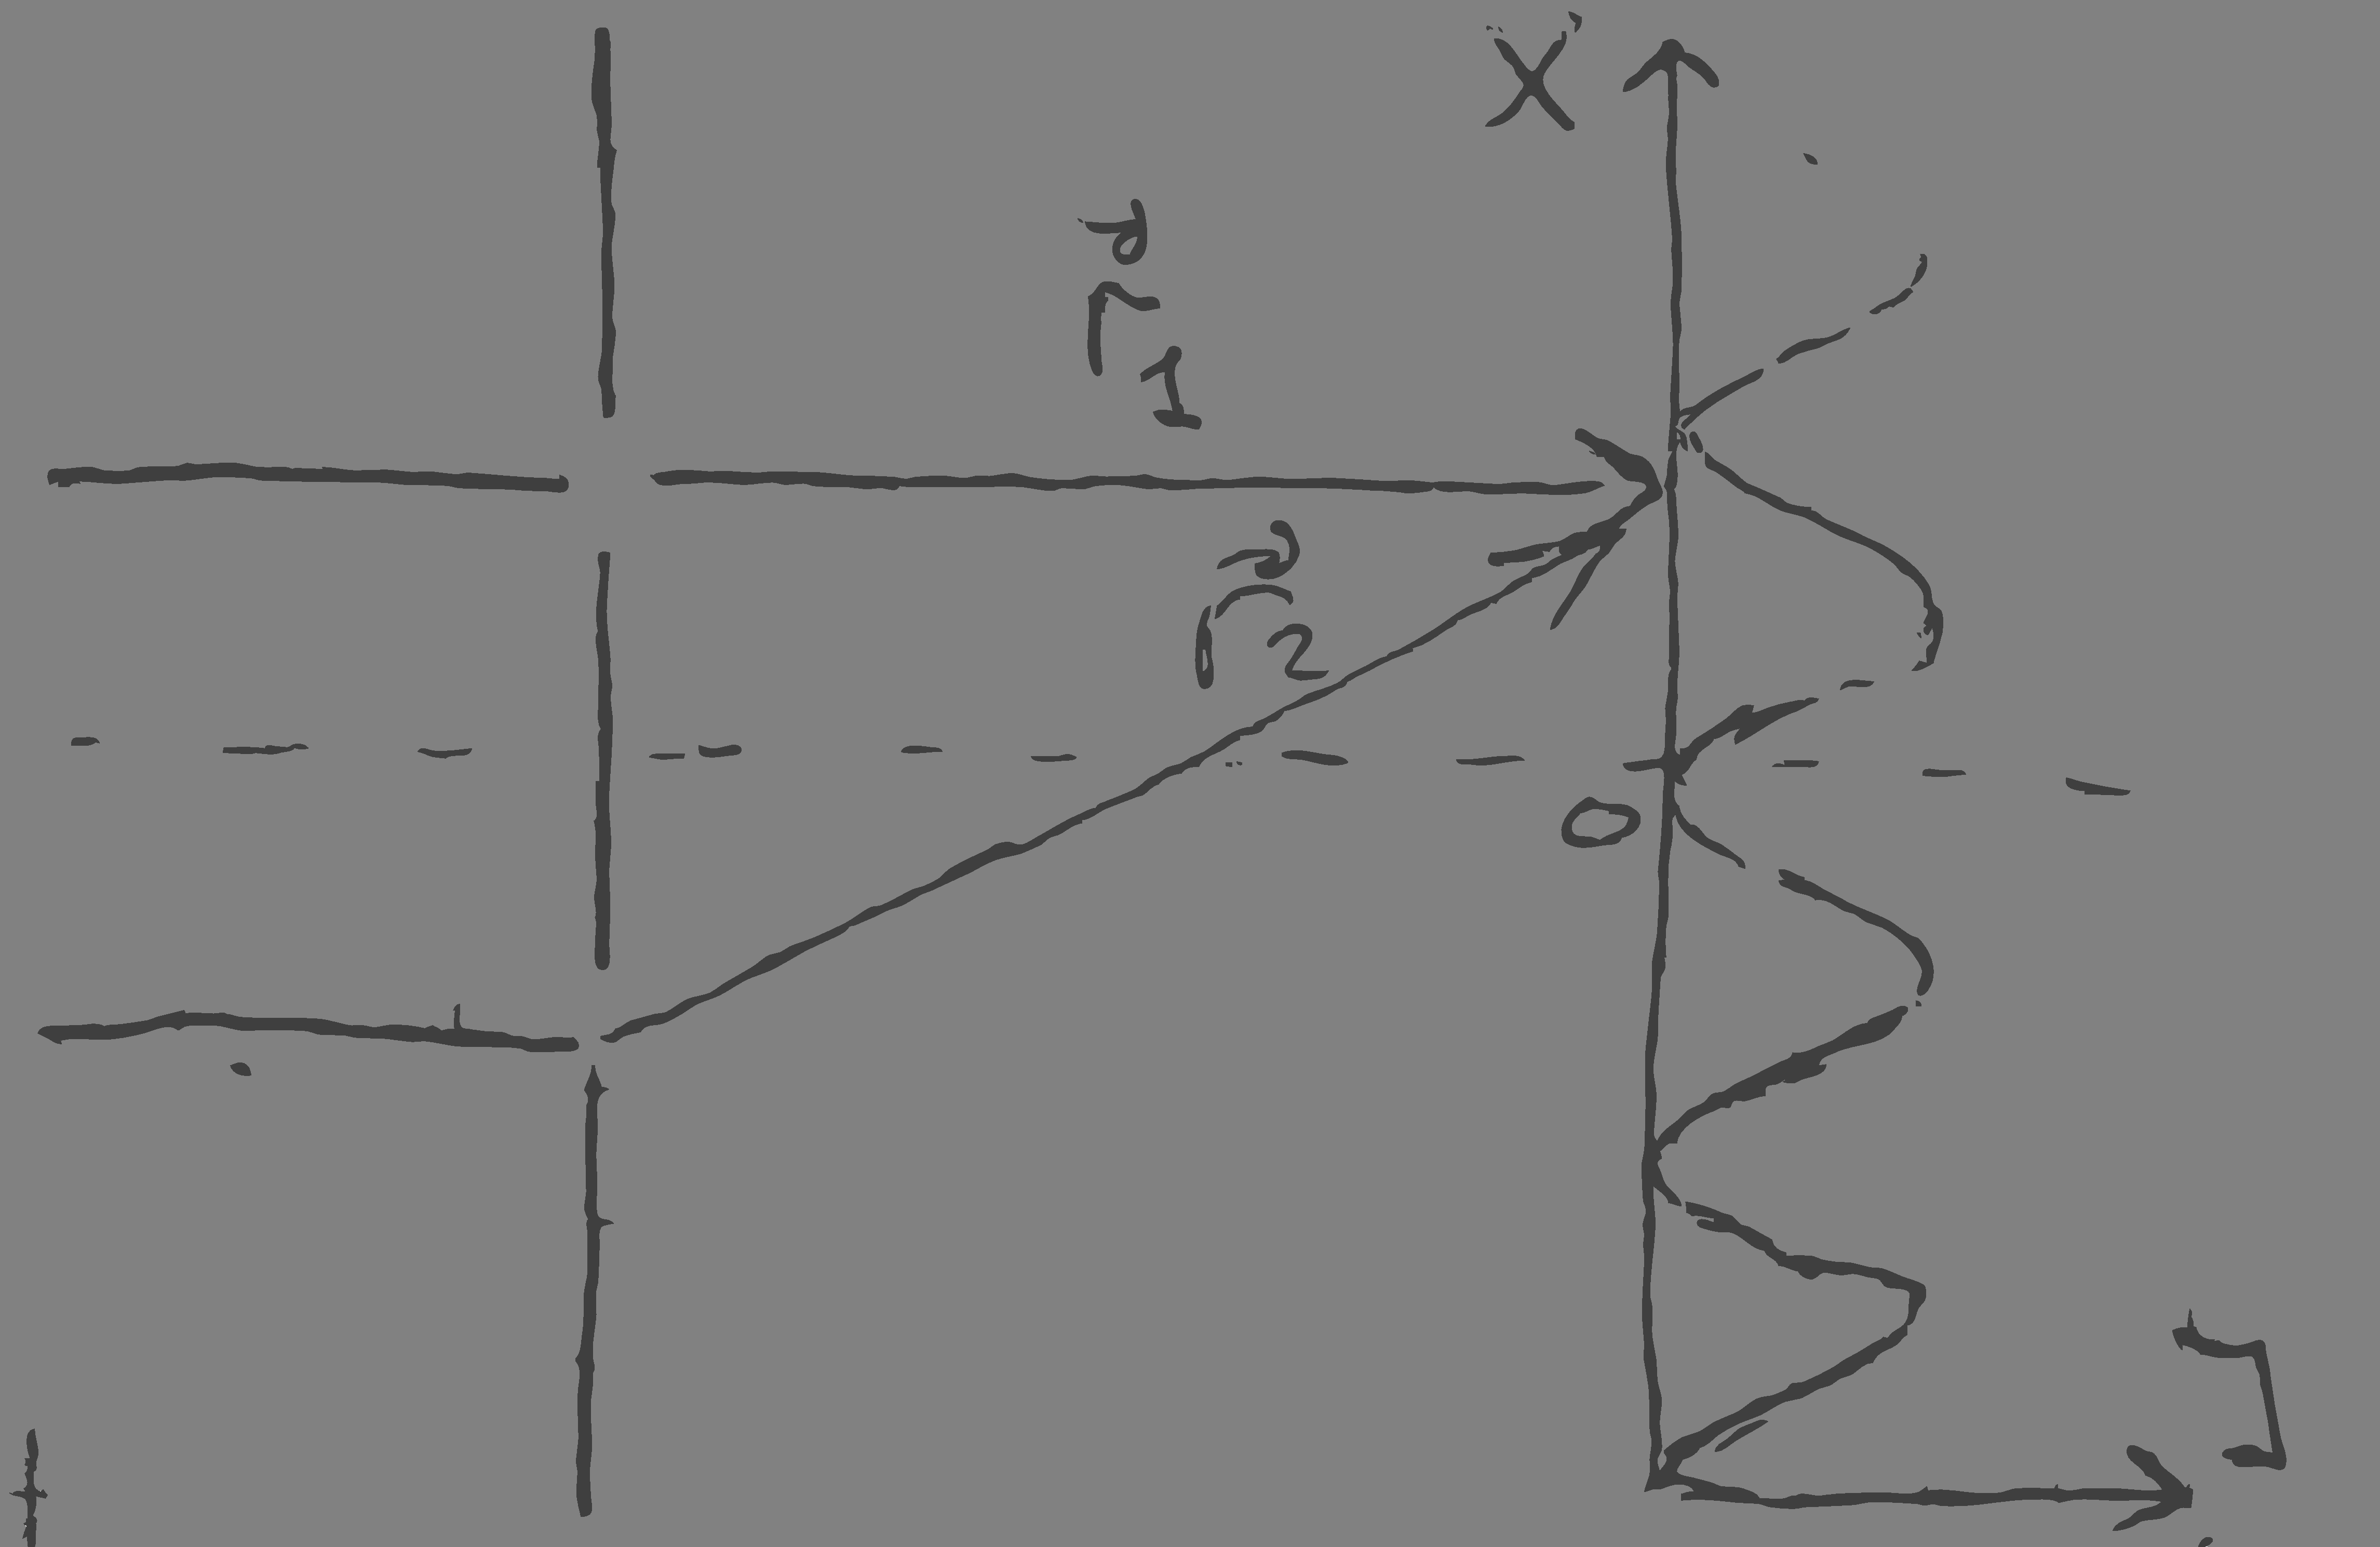
\includegraphics[width=\linewidth]{fig/fig141}
\caption{}
\vspace{-17pt}
\end{wrapfigure}

Предположим, что есть два состояния квантовой системы $\Psi_1$ и $\Psi_2$.
Тогда, по принципу суперпозиции существует состояние $\Psi_3=c_1\Psi_1+c_2\Psi_2$,где
$c_1$ и  $c_2$-- комплексно значные величины, называемые амплитудами вероятности. $\Psi_3$ принимает состояние №1 с вероятностью $|c_1^2|$ и состояние №2 с вероятностью $|c_2|^2$. То есть при сложении двух волновых функций мы не получаем чего-то третьего, а получаем либо состояние №1 с вероятностью $|c_1^2|$, либо №2 с вероятностью $|c_2^2|$.

Одним из наблюдаемых следствий является прохождение электрона через две близко расположенные щели. Если две щели открыты одновременно, то на экране наблюдается интерференционная картина. Это объясняется тем, что электрон находится в суперпозиции состояний.
\begin{equation}
	\Psi(\vec{r},t)=\qty[\Psi_1(\vec{r})+\Psi_2(\vec{r})]\cdot\exp\qty(-\frac{iEt}{\hbar})
\end{equation}
Плотность вероятности нахождения электрона вблизи точки $(\vec{r},t)$ равна:
\begin{gather*}
	|\Psi(\vec{r},t)|^2=|\Psi_1(\vec{r})+\Psi_2(\vec{r})|^2=|\Psi_1(\vec{r},t)|^2+
	|\Psi_2(\vec{r},t)|^2+\qty(\Psi_1^*\Psi_2+\Psi_1\Psi_2^*)=\\
	|\Psi_2(\vec{r},t)|^2+|\Psi_1(\vec{r},t)|^2+2|\Psi_1|\cdot|\Psi_2|\cos(\phi_1-\phi_2)
\end{gather*}

Последнее слагаемое -- интерференционный член. Каждый электрон интерферирует сам  с собой, так как он вошел частично в каждую волну и невозможно точно сказать через какую из щелей он проходит.

\subsubsection{\textcolor{red} {Сформулируйте, что такое дискретный и непрерывный спектры. Каковы волновые
функции, как они нормируются.} }

\subsubsection{\textcolor{red} {Запишите общее решение нестационарного уравнения Шредингера с помощью
разложения по стационарным состояниям} }
